\chapter{ADHD}

\label{ch:ADHD}





ADHD is one of the most serious mental dysfunctions afflicting children and teenagers (there are also subtypes of ADHD but all forms of ADHD are here considered in its general form). It includes a set of patterns associated with inattention, impulsivity and hyperactivity, as the APA defines: ``The essential feature of attention-deficit/hyperactivity disorder (ADHD) is a persistent pattern of inattention and/or hyperactivity-impulsivity that interferes with functioning or development. Inattention manifests behaviorally in ADHD as wandering off task, lacking persistence, having difficulty sustaining focus, and being disorganized and is not due to defiance or lack of comprehension. Hyperactivity refers to excessive motor activity (such as a child running about) when it is not appropriate, or excessive fidgeting, tapping, or talkativeness. In adults, hyperactivity may manifest as extreme restlessness or wearing others out with their activity. Impulsivity refers to hasty actions that occur in the moment without forethought and that have high potential for harm to the individual (e.g., darting into the street without looking).'' \citep{dsm-american}. 



Today there exist many types of treatment, although the main efforts of medicine and psychology are directed to the strict drug-based therapy. In this chapter, will be discussed some general features of children and teenagers afflicted by this disorder, like symptoms, common problems and diagnosis. After that, it will be presented the fundamentals of Stroop Effect, a psychological mechanism related to ADHD, that is used by us to structure the proposed application. The Stroop Effect is correlated to the Stroop Test an psychological procedure used to identify ADHD. In the end, we assemble articles of ADHD children-directed projects of gamification, which contribute to the purpose of this work. 





\section{ADHD Features in Childhood and in Teenage}



Science yet ignores the existence of physiological characteristics and symptoms that are associated with strong disturbances in frontal segment of the brain, a region that is responsible for many neural activities linked to attention and coordination movements. Its symptoms may vary a little. However, the American Psychiatric Association defines the DSM-5 the most usual like frequent failing to focus to details or excessive talking \citep{association2013dsm, Ahma-2013}. Some scholars believe its causes are genetic only, but others disagree in this point suggesting there are also influence of environmental reasons \citep{ADHDDay}. There is no consensus toward this issue. As causality of ADHD is not the subject of present graduate thesis, it is necessary to let this aside by now. In order to define more precisely, what the main features of ADHD are, one needs to recognize some aspects:



``The disorder is also reflected in impairment in will or the capacity to control the child’s own behavior relative to the passage of time, that is, to keep future goals and consequences in mind. It is not, as other books will tell you, just a matter of being inattentive and overactive. It is not just a temporary state that will be outgrown in most cases, a trying but normal phase of childhood. It is not caused by parental failure to properly discipline or raise the child, and it is not a sign of some sort of inherent “badness” or moral failing of the child. ADHD is real: a real disorder, a real problem, and often a real obstacle. It can be heartbreaking and nerve- wracking when not treated properly'' \citep{RBarkley}.



In 2010, 10 million individuals with maximum age of 18 years old have been suffering with ADHD around the world \citep{Psychoanalytic}. At the same time, the consumption of psychiatric medicines to treat this disease has also grew intensively  \citep{Psychoanalytic}. Although this psychological disturbance was first described by a German doctor early in 1790´s there is no permanent and 100\% -efficient mean of treatment. In most of cases it is limited to exclusive use of amphetamines which are associated to severe side effects or may show itself inefficient at long run  \citep{Psychoanalytic}. But its real extension  could be even larger, because people usually  do not understand ADHD main characteristics:



``ADHD is underdiagnosed in most populations, with 40–60\% of such children in any given community in the United States not being diagnosed or treated. But most children do show occasional signs of inattention, over activity, or impulsiveness. What distinguishes children with ADHD from other children is the far greater frequency and severity with which these behaviors are demonstrated and the far greater impairment children with ADHD are likely to experience in many domains of life'' \citep{RBarkley}.



In order to reduce the present way of treatment based almost only in drugs, some physicians and psychologists are suggesting alternatives, including ludic or playing treatments \citep{Psychoanalytic, brainGames}. But, how can one offer this by granting the quality and, at the time, targeting most of affected people at low costs? An reasonable answer lies in mobile computing. Nowadays, speaking only about Brazilian market \citep{idcTablets}, smartphones and tablets are the majority of computing machines, about 150 hundred million, 90\% of them running with android operating system, to a population of 200 hundred million people\citep{idcTablets}), and this may be the mean to achieve ADHD children with the lowest costs. 





\begin{figure}[htp]

	\begin{center}

		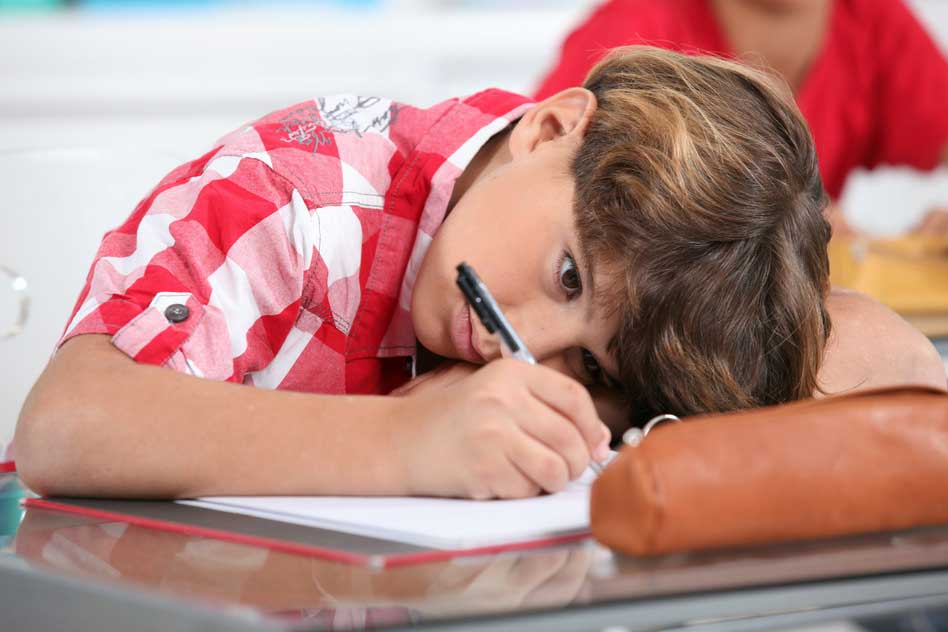
\includegraphics[scale=0.35]{chapters/adhd/img/adhd_child.jpeg}

		\caption{Situation common for ADHD children: their behavioral specificities generally affects negatively its academic capacities. They generally lose their concentration and use to sit without the regular posture to do their homework \citep{child_example}.}

		\label{child}

	\end{center}

\end{figure}



These are the reasons to develop the proposed gamified application, Memory Stroop, which is designed for android mobile devices in order to offer (oferecer o que? Seria oferecer ajuda? – offer help -) to ADHD children. However in order to understand how the game really ought to aid ADHD children it is necessary understanding, firstly, the psychological paradigm in that the game was based, the previous games used on the same purpose that have been presented in literature and, finally, what is the paradigm of gamification used to sustain the game, the Stroop Test, subject of the next chapter. 





\section{Stroop Effect}



The Stroop effect is a psychological phenomenon which happens when human mind and coordination enters in a state of delay in reaction time to perform some task upon conflicting stimuli  condition, for example, reading aloud the name of colors written in different inks from the word representing color. Its name derives from John Ridley Stroop, the first psychologist to develop a solid theory about this phenomenon and to design tests for it, both presented in a scientific article in 1930's \citep{Studies1935}. This test is still employed in many areas of psychology, sometimes with modifications like its Stroop-Gonden modality, particularly interesting for us. It is one of powerful tools to ADHD diagnosis and because of that the base of our gamified implementation.



Before John Ridley Stroop, many researches have tried to explain why the same person tends to perform similar intellectual actions (but with different inputs) in average times so distant. For example, in 1886 James McKeen Cattell published an academic study to show that someone lasts more seconds to say that an object was red than to read aloud the word `red' on a card. But Stroop is appointed as the first to purpose an experiment mixing ink color identification stimulus with reading aloud a different name \citep{macleod}. 



In fact his experiment has three stages well defined: neutral combination between ink colors and color names, congruent combination and incongruent (in figure \ref{stroop} we see the last of three moments of Stroop original experiment). Each moment has its own characteristics and results as it follows. It is important to examine each one, for after, present general conclusions of stroop. 



\begin{enumerate}

\item step: Neutral mixing. In this part, there is only a list of colors printed all in black ink, a neutral color. The intention is to store data performing time to read aloud all words for comparing with two other stages.



\item step: Congruent combination between ink and word. Neutral cards are substituted by cards with words printed with the same color. The average time to read aloud all words is shorter than in the first step. John R. Stroop explains this by the existence of semantic congruence between pure visual stimulus (color ink) and which facilitates mental activities. Years after, other psychologists substituted color names by sequences of colored `X' characters in this stage. In this modified stage the test taker must say the name of color ink of sequence of `X' characters. The congruent effect was, in the latter case, put aside.



\item step: Incongruent combination. This is the main stage. Now cards containing color word are printed in contrasting ink colors Semantic like the word `red' printed in yellow color ink (any person should say only `yellow' instead the written name `red'). The test taker must say only ink color names. Comparing with the average time in first step, the time in this step was drastic lower. This is attributed to an mental context of semantic interference between symbols and concepts by the author.



\end{enumerate}



The general conclusions of three parts of Stroop's experiment may be summarized in follow manner: congruent stimuli (ink name) could facilitate mental activities as conflicting ought to difficult their functioning. After Stroop analysis, a lot of authors have proved that people having attention disturbs and hyperactivity like ADHD children has a particular lower performance.



\begin{figure}[htp]

\begin{center}

  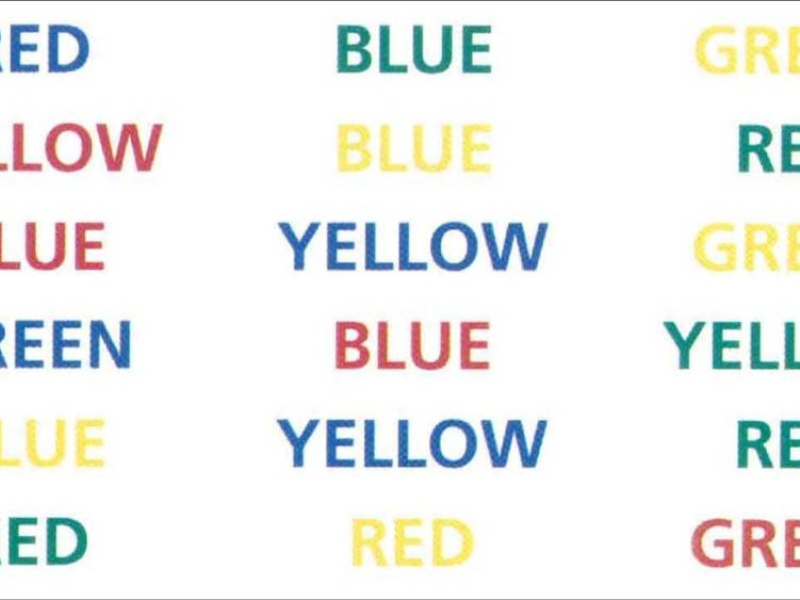
\includegraphics[width=8cm]{chapters/adhd/img/stroop.jpeg}

  \caption{Example of the third stage of test of Stroop in its origin form \citep{iStroop}.}

  \label{stroop}

\end{center}

\end{figure}





Although there are many other applications in psychology, with this test, a psychologist or psychiatric can identify problems in attention, coordination, concentration and inhibitory control -- typical problems of ADHD patients, who  massively fail particularly in the third phase of Stroop experiment \citep{lansbergen}. Although Colors has some specific implementations, which are presented in next chapter, the game was inspired by the Stroop-Golden modality in order to identify and improve ADHD patients' health.



We understands it is possible to use Stroop experiments not only to detect ADHD but also to treat that mental disorder. As MacLeod et al underscore,  John R. Stroop was aware of it: `Experiment 3 also explored the impact of practicing color naming on the development of interference in word reading.  Comparison of a pretest and a post-test where subjects read words in incongruent colors showed that the intervening 8 days of practice introduced interference into word reading (from 19.4 s before to 34.8 s after), but that this newly developed interference quickly disappeared in a second post-test (22.0 s).' \citep{macleod}. In this way continuous practice could benefit capabilities of test takers.



To achieve this end we have chose the Golden-Stroop modality of this psychological test. In this modality the test taker does not use reading name of colors aloud (a controversial feature for some authors \citep{macleod}) and the tests are made in different approach of conflicting stimuli because there is a limited time of 45 seconds to perform tasks counting quantity of mistakes and successes (instead of mean time to perform the test, as it was purposed originally by John Stroop in his own version of test) \citep{goldencj}. This approach is the basis of our application or, at least, of initial game levels of it.



\section{Use of Computing for Play Therapy involving ADHD Children}



There is a relatively considerable number of scientific works about play therapy directed ADHD patients, in particular, children. Some of them emphasize the importance of computing in diagnosis and therapy by coordinating computing and psychology. This graduate thesis follows these articles, besides none of the selected articles presents an application based extensively on the Stroop Effect paradigm discussed in previous section. 



The relevance and role of games (not specifically electronic games, but in a larger sense) for treating ADHD in earliest ages \citep{Psychoanalytic}. In this article, it is discussed about the role of playful therapy methods, which are presented as effective alternative to strict medicine-based one. Although no mention to gamified application is detected in that article, we found useful theoretical foundations to play therapy in it. These foundations allow us to make some mechanisms to treat the ADHD-afflicted children.



In Brazil, computer scientists of Federal University of the State of Rio de Janeiro (UNIRIO - Universidade Federal do Estado do Rio de Janeiro) implemented gamified applications for the ADHD and subtypes diagnosis. The study involved a practical experiment with patients. Time and number of right acts were tabulated and submitted to machine learning algorithms of fuzzy logics, whose output classifications may identify ADHD behavior  and type \citep{brasileiros}. However, there are no mention to the therapeutic potential of its application as we are trying to do here. That work offer some basis to our application in the use of game features to extract diagnostics of ADHD children.



Other article uses a normal game, Pok\'{e}mon, in pratical experiment with ADHD-diagnosed children and a control group of non-ADHD-dignosed \citep{ADHDGames}. Along several weeks, the playing yield was quantified and produced two interesting conclusion. First, all the time there is a distance in the quantity of every movement and right movements from two distinct groups is quite perceptible. This evidences a simple game may be used in diagnosis of the intellectual disorder, distance of scores is characterized among two categories. Second, ADHD children's scores are largely improved at the end of the experiment, assuring potentialities of play therapy \citep{ADHDGames}.



There are academic articles produced by psychiatric and psychological staffs, who emphases less in the algorithmic features of application and explore the neurological beneficial effects of using serious games, called also `brain games', by children \citep{brainGames}. This study monitored the cerebral activity ADHD children and teenagers, of various ethnicities, during their playing of a brain game made of a famous enterprise. Its methodology was quantitative and its results show notorious improvements in frontal lobe of brain activity, associated with symptoms attention and hyperactivity disorder. We do not seek to employ any physiological monitoring during our experiments but it is important to keep in mind that eventual quantitative improvement in ADHD children scores in our game are related with this major neural context. 



Lastly, there is another article \citep{design} that uses the qualitative methodology employed by observing reactions of a fully gamified application, without levels or final aims. The child plays exploring a magic world -- with many 3D landscapes and mechanisms -- and can choose which way to follow and which activities, among many possibilities. Authors' intentions lies in the emphasis in developing creativity and coordination without frustration of too strict rules of playing. This application has some similarities with ours namely in their emphasis in design stimuli of interface, that in both cases was planned to let usability the most fanciful as possible \citep{design}. That work had influenced us in order to put more attention in graphic interface features.



\section{Memory Stroop: Implementing a System to Explore the Correlation between Memory and ADHD}



The proposed application is designed to treat memory complications of the studied disturb. In many ways, attention and memory complements each other, because mental concentration requires all mental functions working well, so far so good, two of main symptoms of inattention component presented by DSM-V, symptoms g. and i., talks about it: ``g. Often loses things necessary for tasks or activities (e.g., school materials, pencils, books, tools, wallets, keys, paperwork, eyeglasses, mobile telephones).  [...] i. Is often forgetful in daily activities (e.g., doing chores, running errands; for older adolescents and adults, returning calls, paying bills, keeping appointments).'' \cite{dsm-american}.

Memory faults are common in patients' daily life, mainly the working memory, which is defined as memory of related of coordination and execution of immediate tasks, but not only of short-term duration as prior studies emphasized, according to relatively recent approaches \citep{working_memory}. There is evidence that training could improve working memory of ADHD children \citep{adhd_memory}. In this way, the proposal of gamification in this graduate thesis combine a common memory game engine with the Stroop Effect colors scheme. The psychological literature has indicated the application  of Stroop Effect to working memory, but without an approach of gamification \citep{Debr-2002}. By combining them, it is possible to train working memory. More details about the proposed gamification lie in chapter \ref{ch:development}.





\section{Summary}



As a serious psychological disturb which afflicts millions of children, teenagers and even adults around the World, ADHD requires more and more resources to combat its symptoms and improve damaged skills and life conditions of its patients. The Stroop Effect and correlated Stroop Test are relevant measures of identification for attention and hyperactivity problems. As the working memory is a core mental skill affected by ADHD, the coordination with memory and attention.
